\documentclass{article} % For LaTeX2e
\usepackage{nips15submit_e,times}
\usepackage{hyperref}
\usepackage{url}
\usepackage{amsmath}
\usepackage{color}
\usepackage{cite}
\usepackage{epsfig, graphics}
%\documentstyle[nips14submit_09,times,art10]{article} % For LaTeX 2.09


\title{Predicting Movies Rating with Cold-Start}

\author{
Supasorn Suwajanakorn, Kanit Wongsuphasawat \\
% \thanks{ Use footnote for providing further information
% about author (webpage, alternative address)---\emph{not} for acknowledging
% funding agencies.} \\
Computer Science \& Engineering\\
University of Washington\\
\texttt{\{supasorn,kanitw\}@cs.washington.edu} \\
}

% The \author macro works with any number of authors. There are two commands
% used to separate the names and addresses of multiple authors: \And and \AND.
%
% Using \And between authors leaves it to \LaTeX{} to determine where to break
% the lines. Using \AND forces a linebreak at that point. So, if \LaTeX{}
% puts 3 of 4 authors names on the first line, and the last on the second
% line, try using \AND instead of \And before the third author name.

\newcommand{\fix}{\marginpar{FIX}}
\newcommand{\new}{\marginpar{NEW}}
\newcommand{\todo}[1]{\textcolor{red}{TODO: #1}}
\newcommand{\red}[1]{\textcolor{red}{#1}}
\newcommand{\U}{U}
\newcommand{\M}{M}

\nipsfinalcopy % Uncomment for camera-ready version

\begin{document}

\maketitle

% \begin{abstract}
% Write abstract here
% \end{abstract}

\section{Problem \& Dataset}

Our goal is to predict movie ratings for each user based on previous ratings and movie metadata which includes official genres and user-provided short tags.  Specifically, we plan to implement a learning model based on matrix factorization~\cite{koren:matrix} that addresses the following problems:

\textbf{1) Cold-Start Problem.}  A common problem for matrix factorization-based method for collaborative filtering is the inability to address unseen items (movies in our case) or users.  We aim to address this problem by using a hybrid model combining matrix factorization and content-based filtering techniques using metadata as features.  To address high dimensionality, we plan to compress the dimensionality of tags using hash-kernel techniques~\cite{shi:hashkernels} or constrain bilinear weights matrix $V$ in Equation $\ref{eq:estimate}$ to be low-rank.

\textbf{2) Run-time Performance.}  We aim to explore parallelization techniques and frameworks that enable fast learning algorithm.  In our initial work, we experiment with a simple interference-free parallelization scheme for stochastic gradient descent (SGD) which avoids work overriding and can simultaneously utilize all available cores. We plan to implement and compare SGD on a distributed framework such as GraphLab.

% We plan to compare our method with Hogwild method by Niu et al.~\cite{niu:hogwild} that uses a shared-memory model without locks to eliminate the locking overhead.

\textbf{3) Class Imbalance.}  It has been shown that in the general context of link prediction and many learning problems, the bias or imbalance of the output class in the training set adversely affects the accuracy of the final predictor. In this work, we will investigate how sensitive rating imbalance affects the outcome of the movie rating prediction. If the accuracy indeed suffers from such imbalance, we plan to follow \cite{menon:link-prediction} and use a relative loss measure to handle imbalance and directly optimizes AUC curve with a modified loss function. The resulting objective can still be optimized with SGD.

We use the MovieLens 20M\footnote{http://grouplens.org/datasets/movielens/}
as our benchmark dataset.  The dataset contains over 20 million ratings and 465 thousand tags assigned to 27,278 movies by 138,493 users and excludes users who rated fewer than 20 movies. The input rating matrix is sparse since only 0.5\% of the matrix's cells contain values.




\section{Matrix Factorization with Stochastic Gradient Descent}

We first map the relationship between movies, users and ratings
as a matrix factorization problem with an explicit feature model.
Each rating is modeled as a sum of the inner product between a vector of user and movie in the latent space of rank $k$, biases associated with each user and movie ($b_u, b_m$), and a bilinear regression model \cite{gabriel1998generalised}. The estimate of movie $m$'s rating by user $u$ is given by.

\[
  \hat{r}_{um} = \U_u \M_m^T + b_u + b_m + x_u^T V x_m
  \label{eq:estimate}
\]

where $\U_u$ is a rank-$k$ vector that represents row $u$-th of the latent matrix for users $\U$ and $\M_m$ is a rank-$k$ vector that represents row $m$-th of the latent matrix for movies $\M$. $x_u$ and $x_m$ are features associated with user $u$ and movie $m$, and $V$ contains the bilinear weights, which can be constrained to have low-rank by decomposing $V=D + A^TB$ where D is diagonal and $A,B$ are low-rank matrices.

As an initial implementation, we compute the standard matrix factorization without explicit feature on a (20\%) subset of MovieLens dataset. That is, we minimize regularized squared errors on the set of known ratings (discussed in lecture).

\begin{align}
  \min_{\U,\M} \sum_{r_{um}} (\U_u \cdot \M_m^T - r_{um})^2
  + \lambda_u \|\U\|^2_F + \lambda_m \|\M\|^2_F
\end{align}
To find a solution, we apply stochastic gradient descent using the following update equation:

\begin{align}
\left[\begin{array}{c}
\U_u^{(t+1)}
\\
\M_m^{(t+1)}
\end{array}\right]
& \leftarrow
\left[\begin{array}{c}
(1-\eta_t \lambda_u) \U_u^{(t)} - \eta_t \epsilon_t \M_m^{(t)}
\\
(1-\eta_t \lambda_v) \M_m^{(t)} - \eta_t \epsilon_t \U_u^{(t)}
\end{array}\right]
\label{eq:update}
\end{align}

where $\eta_t$ is the step size at time $t$ which are all currently set to 0.01.

\section{Parallel Stochastic Gradient Descent without Interference}

To speed-up matrix factorization, we develop a parallizing scheme for matrix factorization without inference.
In this paper, we refer to each parallel unit as processor, but the same concept is also applicable for any distributed system environment.

From (\ref{eq:update}), from an observation that the algorithm only updates row $\U_u$ and $M_m$ when rating $r_{um}$ is observed, we can divide the dataset into subsets such that the movies and users in each subset are disjoint and can be independently processed at the same time.

One method is to split the input matrix $R$, both vertically and horizontally
into $p \times p$ submatrices where $p$ is number of processors
(Figure~\ref{fig:split}). We then divide each pass over the entire training
set into $p$ (sub-)iterations. For the first iteration, we distribute $p$ sub
matrices along the diagonal to each processor.  And for subsequent iterations, each processor is assigned the submatrix on the right of the
previously assigned submatrix and warp around to the left-most submatrix if we reach the end. With this assignment, every movie $m$ and every user $u$ updated by processor p in each iteration will not be updated by other processors in the same subiteration.

Advantages of this scheme include a trivial scheduling scheme that does not require complex synchronizations and can fully operate on a single shared memory, and a known deteministic memory locality which helps speed up computation with a proper memory caching. However, one important consideration for this scheme is the load balancing. The distribution of sparse observations in matrix $R$ can be non-uniform leading to imbalanced computational burdens. Remedies for this include subdividing the observation matrix into smaller chucks i.e. $q \times q$ such that $q$ is greater than the number of processors and have a single processor operate on more than one submatrix per subiteration. Another way is to randomly shuffle the rows and columns of the observation matrix. It would be interesting to see how this compares to general graph-based scheduling algorithms such as those in GraphLab.

\begin{figure}[h]
%\framebox[4.0in]{$\;$}
\centering
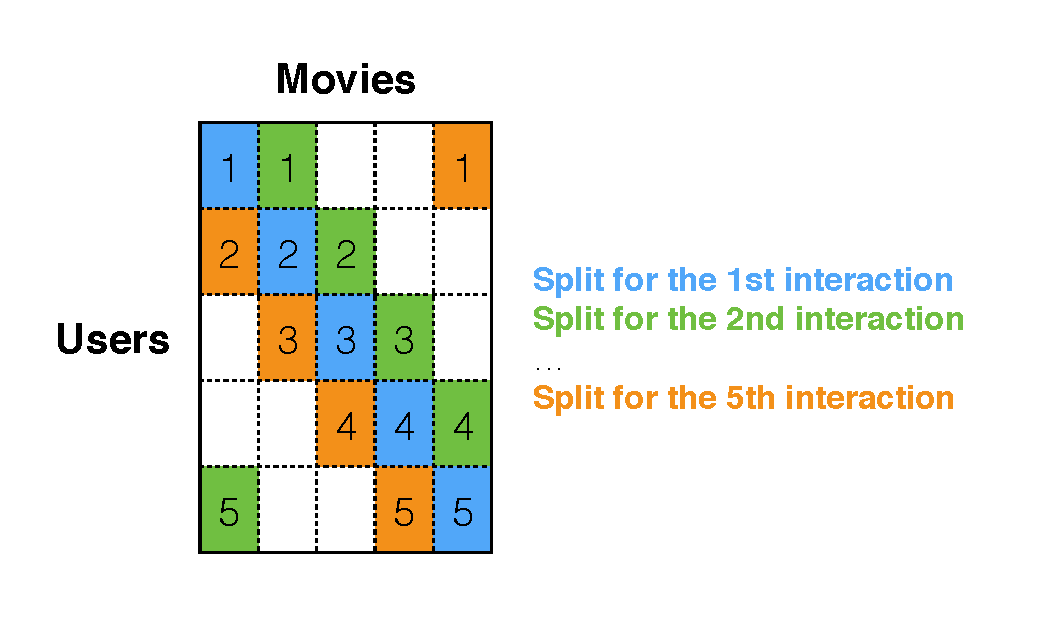
\includegraphics[width=3in]{figures/split.pdf}
\caption{\label{fig:split} Paralellizing the matrix with 5 processors.}
\end{figure}

\section{Implementation}

We implement a matrix factorization in python using numpy and scipy and use python's \texttt{multiprocessing} library to spawn multiple processes with shared read-write memory for the latent variable. The number of processes spawned is set to the number of CPU cores.

Since this is a non-convex optimization, we initialize the latent matrices $U$ and $M$ by drawing a sample from a uniform distribution in the range $[0,\sqrt{\frac{\bar{r}}{0.25k}})$ for each entry in the matrices where $\bar{r}$ is the average rating and $k$ is the matrix rank so that $E[\hat{r}_{um}] = \bar{r}$ after initialization.

\section{Initial Results}

\textbf{Parallel Speed-up.}  Compared to a single-process algorithm, our
parallel version obtains around 20x speed up when run on a 32-core machine. In
principle, the speed should scale up linearly with the number of processes
used. We suspect that this is due to the multiprocess overhead and load
imbalancing and we would hope to see a better speed-up when we run on the
original big dataset.

\textbf{Varying lambda.}  For our preliminary results, we try the simple
matrix factorization problem (no explicit feature) with different
values of $\lambda$ in $\{0, 0.01, \ldots, 0.2\}$. We run this simultaneously
on a GRAIL cluster which consists of nodes with varying cores from 8 to 32. We
limit the maximum number of iterations to 300 and the time it took varies from
4 to 11 hours depending on the machines and their current loads. A plot of
training and testing RMSE's with respect to $\lambda$ is shown in Figure
\ref{fig:rmselambda}. We have not performed a cross-validation to evaluate the
best set of parameters ($\lambda$, latent rank) -- this will be part of our
final work.


\begin{figure}[h]
\centering
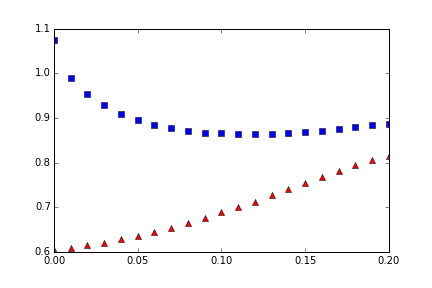
\includegraphics[width=3in]{../plot.png}
\caption{\label{fig:rmselambda} A plot of
training (red triangle) and testing (blue square) RMSE's with respect to $\lambda$ }
\end{figure}

% \section{Next Steps}

% We plan to further find optimal parameters for rank of latent vectors $k$
% (in addition to regularizaiton parameter) using grid search.



% If time allows: other parallezing scheme, temporal dynamics.)

% http://research.yahoo.com/files/kdd-fp074-koren.pdf

% \begin{table}[t]
% \caption{Sample table title}
% \label{sample-table}
% \begin{center}
% \begin{tabular}{ll}
% \multicolumn{1}{c}{\bf PART}  &\multicolumn{1}{c}{\bf DESCRIPTION}
% \\ \hline \\
% Dendrite         &Input terminal \\
% Axon             &Output terminal \\
% Soma             &Cell body (contains cell nucleus) \\
% \end{tabular}
% \end{center}
% \end{table}

\bibliographystyle{abbrv}
\bibliography{paper_supasorn_kanitw}{}

\end{document}